\PassOptionsToPackage{unicode=true}{hyperref} % options for packages loaded elsewhere
\PassOptionsToPackage{hyphens}{url}
%
\documentclass[12pt,]{article}
\usepackage{lmodern}
\usepackage{amssymb,amsmath}
\usepackage{ifxetex,ifluatex}
\usepackage{fixltx2e} % provides \textsubscript
\ifnum 0\ifxetex 1\fi\ifluatex 1\fi=0 % if pdftex
  \usepackage[T1]{fontenc}
  \usepackage[utf8]{inputenc}
  \usepackage{textcomp} % provides euro and other symbols
\else % if luatex or xelatex
  \usepackage{unicode-math}
  \defaultfontfeatures{Ligatures=TeX,Scale=MatchLowercase}
    \setmainfont[]{Times New Roman}
\fi
% use upquote if available, for straight quotes in verbatim environments
\IfFileExists{upquote.sty}{\usepackage{upquote}}{}
% use microtype if available
\IfFileExists{microtype.sty}{%
\usepackage[]{microtype}
\UseMicrotypeSet[protrusion]{basicmath} % disable protrusion for tt fonts
}{}
\IfFileExists{parskip.sty}{%
\usepackage{parskip}
}{% else
\setlength{\parindent}{0pt}
\setlength{\parskip}{6pt plus 2pt minus 1pt}
}
\usepackage{hyperref}
\hypersetup{
            pdftitle={Analysis of drinking water water contaminant occurrence in the northeastern and southeastern United States},
            pdfauthor={Rachel Gonsenhauser},
            pdfborder={0 0 0},
            breaklinks=true}
\urlstyle{same}  % don't use monospace font for urls
\usepackage[margin=2.54cm]{geometry}
\usepackage{longtable,booktabs}
% Fix footnotes in tables (requires footnote package)
\IfFileExists{footnote.sty}{\usepackage{footnote}\makesavenoteenv{longtable}}{}
\usepackage{graphicx,grffile}
\makeatletter
\def\maxwidth{\ifdim\Gin@nat@width>\linewidth\linewidth\else\Gin@nat@width\fi}
\def\maxheight{\ifdim\Gin@nat@height>\textheight\textheight\else\Gin@nat@height\fi}
\makeatother
% Scale images if necessary, so that they will not overflow the page
% margins by default, and it is still possible to overwrite the defaults
% using explicit options in \includegraphics[width, height, ...]{}
\setkeys{Gin}{width=\maxwidth,height=\maxheight,keepaspectratio}
\setlength{\emergencystretch}{3em}  % prevent overfull lines
\providecommand{\tightlist}{%
  \setlength{\itemsep}{0pt}\setlength{\parskip}{0pt}}
\setcounter{secnumdepth}{5}
% Redefines (sub)paragraphs to behave more like sections
\ifx\paragraph\undefined\else
\let\oldparagraph\paragraph
\renewcommand{\paragraph}[1]{\oldparagraph{#1}\mbox{}}
\fi
\ifx\subparagraph\undefined\else
\let\oldsubparagraph\subparagraph
\renewcommand{\subparagraph}[1]{\oldsubparagraph{#1}\mbox{}}
\fi

% set default figure placement to htbp
\makeatletter
\def\fps@figure{htbp}
\makeatother

\usepackage{etoolbox}
\makeatletter
\providecommand{\subtitle}[1]{% add subtitle to \maketitle
  \apptocmd{\@title}{\par {\large #1 \par}}{}{}
}
\makeatother

\title{Analysis of drinking water water contaminant occurrence in the
northeastern and southeastern United States}
\providecommand{\subtitle}[1]{}
\subtitle{\url{https://github.com/rachel-gonsenhauser/Final_Project_Environmental_Data_Analytics}}
\author{Rachel Gonsenhauser}
\date{}

\begin{document}
\maketitle

\newpage
\abstract

\begin{quote}
add text here once finnndinngs clear!!!!
\end{quote}

\newpage
\tableofcontents 
\newpage
\listoftables 
\newpage
\listoffigures 
\newpage

\hypertarget{rationale-and-research-questions}{%
\section{Rationale and Research
Questions}\label{rationale-and-research-questions}}

\begin{quote}
While the EPA establishes standards for 90 drinking water contaminants
by means of the federal Safe Drinking Water Act (SDWA) and its
regulations, public water systems still often struggle to remain in
compliance with such policies (USEPA, 2020). This issue of compliance
with the SDWA can stem from myriad causes, for instance financial
capacity of the water system. This is especially concerning in areas
where geologic conditions and/or anthropogenic activities frequently
introduce contaminants into drinking water supplies. Additionally, some
known contaminants still have yet to be regulated by the EPA, such as
poly- and perfluoroaklyl substances (PFAS), which introduces even more
complexity to the issue of water quality monitoring of drinking water
sources.
\end{quote}

\begin{quote}
This analysis seeks to investigate the co-occurrence of water quality
indicators including arsenic, trihalomethane, uranium, and PFAS, which
originate from both geogenic and anthropogenic sources. Additionally,
given pervasive questions related to environmental justice and how
socioeconomic factors may be related to water quality indicators, this
analysis seeks to examine relationships between water quality indicators
and county-level median household income (MHI) and size of the
population served by a given community water system (CWS), which is
often a proxy for how rural an area is and the financial capacity of a
CWS. Additionally, questions regarding how contaminant occurrence
differs across time and between states are explored.
\end{quote}

\begin{quote}
To narrow the scope of this project, most analyses are targeted to
southeastern region states and northeastern region states. These regions
were chosen given their differences in geology and socioeconmic makeup.
Additionally, individual case studies of Massachusetts and North
Carolina are explored in further depth. As arsenic is present in much of
the underlying geology in New England and other northeastern states,
arsenic data is used is many of the analyses performed. Due to issues of
PFAS data limitations, discussed in more detail in the subsequent
section, analyses using PFAS data are limited.

Specifically, the following questions are explored in this analysis:
Question 1: Do arsenic concentrations vary significantly from state to
state in northeastern and southeastern states? Question 2: Do
socioeconomic factors or the presence of other contaminants predict
arsenic concentrations in Massachusetts and North Carolina? Question 3:
Do PFAS concentrations vary signficantly across time and from state to
state in the United States? Are socioeconomic factors significant
predictors of PFAS concentrations?
\end{quote}

\newpage

\hypertarget{dataset-information}{%
\section{Dataset Information}\label{dataset-information}}

\begin{quote}
Data used for this analysis was downloaded from the Centers for Disease
Control and Prevention (CDC)'s National Environmental Public Health
Tracking Network at Centers for Disease Control and Prevention (CDC)'s
National Environmental Public Health Tracking Network
\url{https://ephtracking.cdc.gov/DataExplorer/\#/}. Output from this
online tool containing geographic and CWS data associated with
individual variables was combined into the final processed dataset used
for this analysis.
\end{quote}

\begin{quote}
The wrangling process entailed taking individual datasets containing
data for arsenic, PFAS, uranium, trihalomethane, and MHI and joining
them into the final processed dataset. Each of these variables had
accompanying data inncluding the year, state, county, and CWS in which
the data was collected for each parameter. As unique county Federal
Information Processing Standards (FIPS) codes were standard across all
individual datasets, this variable was used to join datasets into the
final processed dataset.
\end{quote}

Figure 1: Summary information for processed dataset

\begin{longtable}[]{@{}ll@{}}
\toprule
\textbf{Parameter} & \textbf{Summary}\tabularnewline
\midrule
\endhead
Number of states & 28\tabularnewline
Number of CWSs & 25,583\tabularnewline
Water quality indicators & Arsenic, trihalomethane, uranium,
PFAS\tabularnewline
Socioeconomic variables & Population served by CWS, MHI\tabularnewline
Data collection time span & 1999-2018\tabularnewline
\bottomrule
\end{longtable}

Figure 2: Description of Variables Used in Analyses

\begin{longtable}[]{@{}lll@{}}
\toprule
\begin{minipage}[b]{0.22\columnwidth}\raggedright
\textbf{Column Heading}\strut
\end{minipage} & \begin{minipage}[b]{0.46\columnwidth}\raggedright
\textbf{Variable Description}\strut
\end{minipage} & \begin{minipage}[b]{0.23\columnwidth}\raggedright
\textbf{Data Range}\strut
\end{minipage}\tabularnewline
\midrule
\endhead
\begin{minipage}[t]{0.22\columnwidth}\raggedright
stateFIPS\strut
\end{minipage} & \begin{minipage}[t]{0.46\columnwidth}\raggedright
Federal Information Processing Standard state code\strut
\end{minipage} & \begin{minipage}[t]{0.23\columnwidth}\raggedright
N/A\strut
\end{minipage}\tabularnewline
\begin{minipage}[t]{0.22\columnwidth}\raggedright
State\strut
\end{minipage} & \begin{minipage}[t]{0.46\columnwidth}\raggedright
state measurement was taken in\strut
\end{minipage} & \begin{minipage}[t]{0.23\columnwidth}\raggedright
N/A\strut
\end{minipage}\tabularnewline
\begin{minipage}[t]{0.22\columnwidth}\raggedright
countyFIPS\strut
\end{minipage} & \begin{minipage}[t]{0.46\columnwidth}\raggedright
Federal Information Processing Standard county code\strut
\end{minipage} & \begin{minipage}[t]{0.23\columnwidth}\raggedright
N/A\strut
\end{minipage}\tabularnewline
\begin{minipage}[t]{0.22\columnwidth}\raggedright
County\strut
\end{minipage} & \begin{minipage}[t]{0.46\columnwidth}\raggedright
county measurement was taken in\strut
\end{minipage} & \begin{minipage}[t]{0.23\columnwidth}\raggedright
N/A\strut
\end{minipage}\tabularnewline
\begin{minipage}[t]{0.22\columnwidth}\raggedright
Year\strut
\end{minipage} & \begin{minipage}[t]{0.46\columnwidth}\raggedright
year measurement was taken in\strut
\end{minipage} & \begin{minipage}[t]{0.23\columnwidth}\raggedright
N/A\strut
\end{minipage}\tabularnewline
\begin{minipage}[t]{0.22\columnwidth}\raggedright
Arsenic\_ugL\strut
\end{minipage} & \begin{minipage}[t]{0.46\columnwidth}\raggedright
mean arsenic concentration (micrograms per liter)\strut
\end{minipage} & \begin{minipage}[t]{0.23\columnwidth}\raggedright
1-2,422 micrograms/liter\strut
\end{minipage}\tabularnewline
\begin{minipage}[t]{0.22\columnwidth}\raggedright
PWS.ID\strut
\end{minipage} & \begin{minipage}[t]{0.46\columnwidth}\raggedright
Public Water System Identification Number\strut
\end{minipage} & \begin{minipage}[t]{0.23\columnwidth}\raggedright
N/A\strut
\end{minipage}\tabularnewline
\begin{minipage}[t]{0.22\columnwidth}\raggedright
CWS.Name\strut
\end{minipage} & \begin{minipage}[t]{0.46\columnwidth}\raggedright
Community Water System Name\strut
\end{minipage} & \begin{minipage}[t]{0.23\columnwidth}\raggedright
N/A\strut
\end{minipage}\tabularnewline
\begin{minipage}[t]{0.22\columnwidth}\raggedright
Population.Served\strut
\end{minipage} & \begin{minipage}[t]{0.46\columnwidth}\raggedright
number of people served by CWS\strut
\end{minipage} & \begin{minipage}[t]{0.23\columnwidth}\raggedright
0-8,271,000 people\strut
\end{minipage}\tabularnewline
\begin{minipage}[t]{0.22\columnwidth}\raggedright
MHI\strut
\end{minipage} & \begin{minipage}[t]{0.46\columnwidth}\raggedright
median household income (\$)\strut
\end{minipage} & \begin{minipage}[t]{0.23\columnwidth}\raggedright
\$16,435-\$113,336\strut
\end{minipage}\tabularnewline
\begin{minipage}[t]{0.22\columnwidth}\raggedright
PFAS\_ppt\strut
\end{minipage} & \begin{minipage}[t]{0.46\columnwidth}\raggedright
PFAS conncentration (parts per trillion)\strut
\end{minipage} & \begin{minipage}[t]{0.23\columnwidth}\raggedright
1-60 ppt\strut
\end{minipage}\tabularnewline
\begin{minipage}[t]{0.22\columnwidth}\raggedright
TTHM\_ugl\strut
\end{minipage} & \begin{minipage}[t]{0.46\columnwidth}\raggedright
mean trihalomethane concentration (micrograms per liter)\strut
\end{minipage} & \begin{minipage}[t]{0.23\columnwidth}\raggedright
0-219.20 micrograms/liter\strut
\end{minipage}\tabularnewline
\begin{minipage}[t]{0.22\columnwidth}\raggedright
Uranium\_ugL\strut
\end{minipage} & \begin{minipage}[t]{0.46\columnwidth}\raggedright
mean uranium concentration (micrograms per liter)\strut
\end{minipage} & \begin{minipage}[t]{0.23\columnwidth}\raggedright
0-379.10 micrograms/liter\strut
\end{minipage}\tabularnewline
\begin{minipage}[t]{0.22\columnwidth}\raggedright
MCL\_TTM\strut
\end{minipage} & \begin{minipage}[t]{0.46\columnwidth}\raggedright
whether MCL for trihalomethanes is exceeded\strut
\end{minipage} & \begin{minipage}[t]{0.23\columnwidth}\raggedright
N/A\strut
\end{minipage}\tabularnewline
\begin{minipage}[t]{0.22\columnwidth}\raggedright
MCL\_Uranium\strut
\end{minipage} & \begin{minipage}[t]{0.46\columnwidth}\raggedright
whether MCL for uranium is exceeded\strut
\end{minipage} & \begin{minipage}[t]{0.23\columnwidth}\raggedright
N/A\strut
\end{minipage}\tabularnewline
\begin{minipage}[t]{0.22\columnwidth}\raggedright
MCL\_Arsenic\strut
\end{minipage} & \begin{minipage}[t]{0.46\columnwidth}\raggedright
whether MCL for arsenic is exceeded\strut
\end{minipage} & \begin{minipage}[t]{0.23\columnwidth}\raggedright
N/A\strut
\end{minipage}\tabularnewline
\bottomrule
\end{longtable}

\begin{quote}
Figure 1 provides a high level summary of the data provided in the
processed dataset. It should be noted that PFAS data was only available
for 2013-2015. For ease of analysis, this date range was changed to 2014
during the raw dataset wrangling process to create a common annual unit
of analysis for all variables. Figure 2 provides descriptions of all
variables included in the processed dataset with data ranges provided
for continuous variables.
\end{quote}

\newpage

\hypertarget{exploratory-analysis}{%
\section{Exploratory Analysis}\label{exploratory-analysis}}

\hypertarget{data-exploration-for-southeastern-states}{%
\subsection{Data Exploration for Southeastern
States}\label{data-exploration-for-southeastern-states}}

Table 3: Summary Statistics for Southeastern State Variables

\begin{longtable}[]{@{}lll@{}}
\toprule
\textbf{Parameter} & \textbf{Mean} & \textbf{Data Range}\tabularnewline
\midrule
\endhead
MHI & \$40,848 & \$16,435-\$92,097\tabularnewline
Population served by CWS & 14,893 people & 0-2,300,000
people\tabularnewline
Arsenic & 410.6 micrograms/liter & 1.0-2,395.0
micrograms/liter\tabularnewline
Uranium & 0.681 micrograms/liter & 0-23.84
micrograms/liter\tabularnewline
PFAS & 31.71 ppt & 7.0-59.00 ppt\tabularnewline
Trihalomethane & 17.47 micrograms/liter & 0-80.00
micrograms/liter\tabularnewline
\bottomrule
\end{longtable}

\begin{quote}
Southeastern states examined include counties with a large range of
income levels and water system sizes; additionally, arsenic
concentrations vary more than any other contaminant examined (Table 3).
\end{quote}

\begin{figure}
\centering
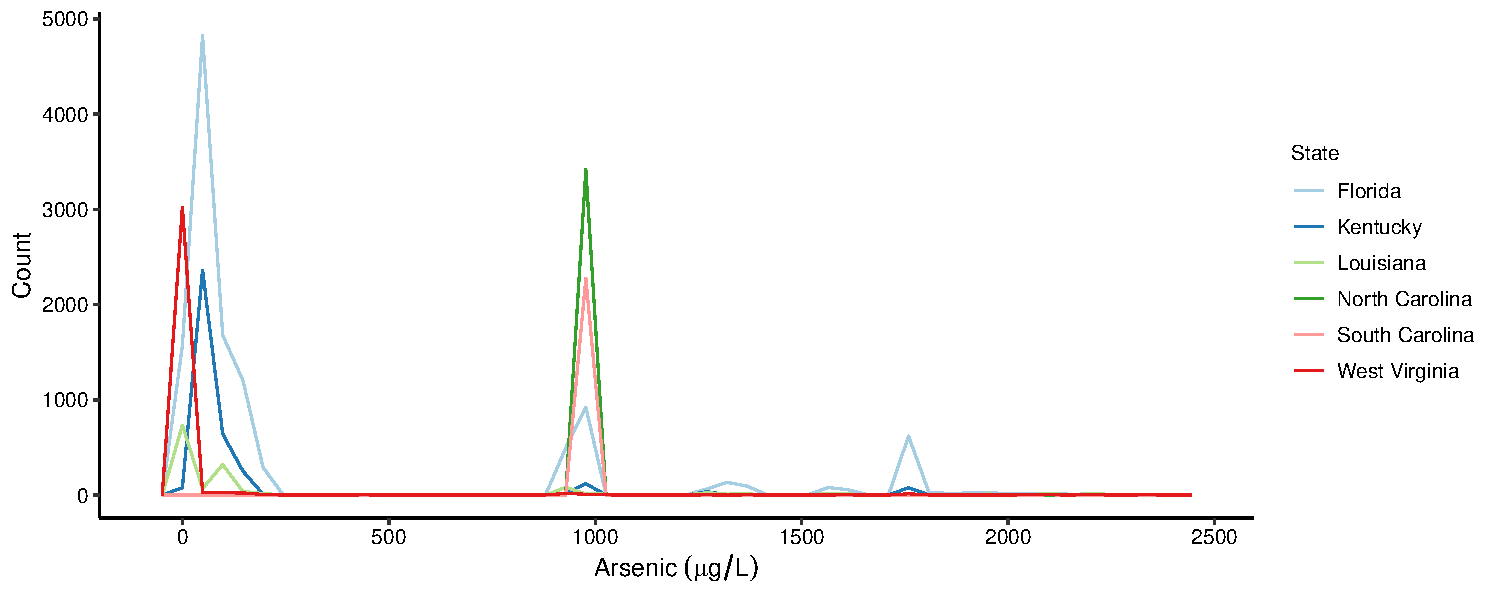
\includegraphics{Project_Template_files/figure-latex/figs-1.pdf}
\caption{Frequency of Arsenic Concentration Data in Southeastern
states.}
\end{figure}

\begin{verbatim}
## Warning: Removed 26290 rows containing non-finite values (stat_bin).
\end{verbatim}

\begin{figure}
\centering
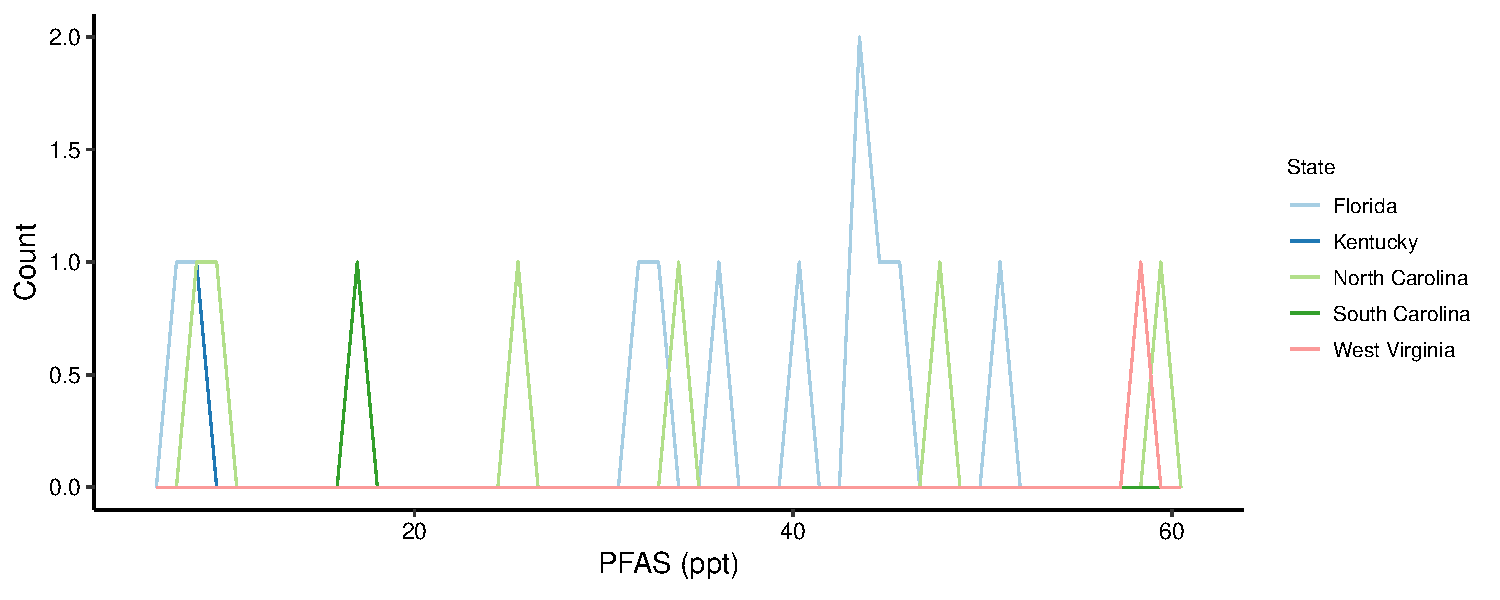
\includegraphics{Project_Template_files/figure-latex/figs2-1.pdf}
\caption{Frequency of PFAS Concentration Data in Southeastern states.}
\end{figure}

\begin{quote}
Insert text here explaining what these exploratory plots
say!!!!**********
\end{quote}

\newpage

\hypertarget{data-exploration-for-northeastern-states}{%
\subsection{Data Exploration for Northeastern
States}\label{data-exploration-for-northeastern-states}}

Table 3: Summary Statistics for Northeastern State Variables

\begin{longtable}[]{@{}lll@{}}
\toprule
\textbf{Parameter} & \textbf{Mean} & \textbf{Data Range}\tabularnewline
\midrule
\endhead
MHI & \$54,513 & \$26,323-\$113,336\tabularnewline
Population served by CWS & 13,791 people & 0-8271000
people\tabularnewline
Arsenic & 359.2 micrograms/liter & 1.0-2,2,422.0
micrograms/liter\tabularnewline
Uranium & 1.75 micrograms/liter & 0-43.00
micrograms/liter\tabularnewline
PFAS & 29.76 ppt & 3-60.00 ppt\tabularnewline
Trihalomethane & 10.37 micrograms/liter & 0-134.10
micrograms/liter\tabularnewline
\bottomrule
\end{longtable}

\begin{quote}
Summary statistics for the northeastern United States indicate the the
median household income is higher than that inn the southeast and that
while the average water system size is similar across regions, the
northeast has systems to serve upwards of 8 million people, as compared
to a maxiumum size of 2 million people in the southeast (Tables 3 and
4). Ranges and average values for water quality indicators were
relatively similar in both regions (Tables 3 and 4).
\end{quote}

\begin{figure}
\centering
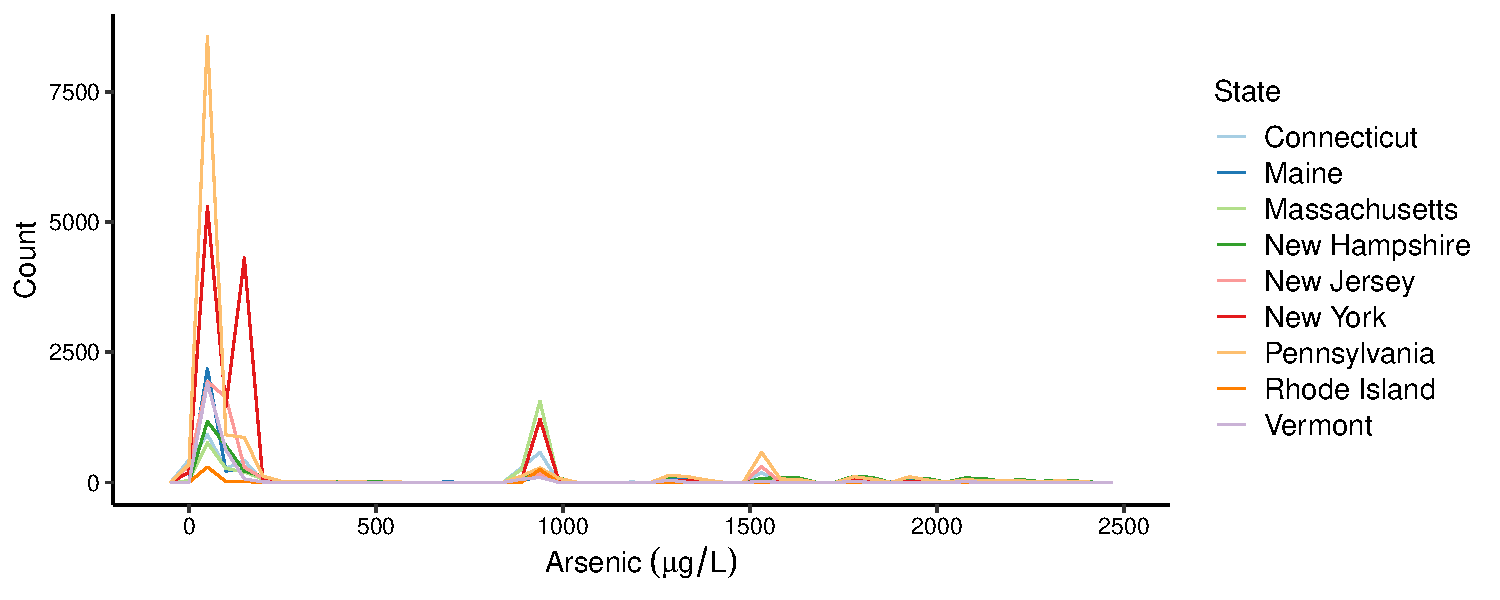
\includegraphics{Project_Template_files/figure-latex/figs3-1.pdf}
\caption{Frequency of Arsenic Concentration Data in Noutheastern
states.}
\end{figure}

\begin{verbatim}
## Warning: Removed 26290 rows containing non-finite values (stat_bin).
\end{verbatim}

\begin{figure}
\centering
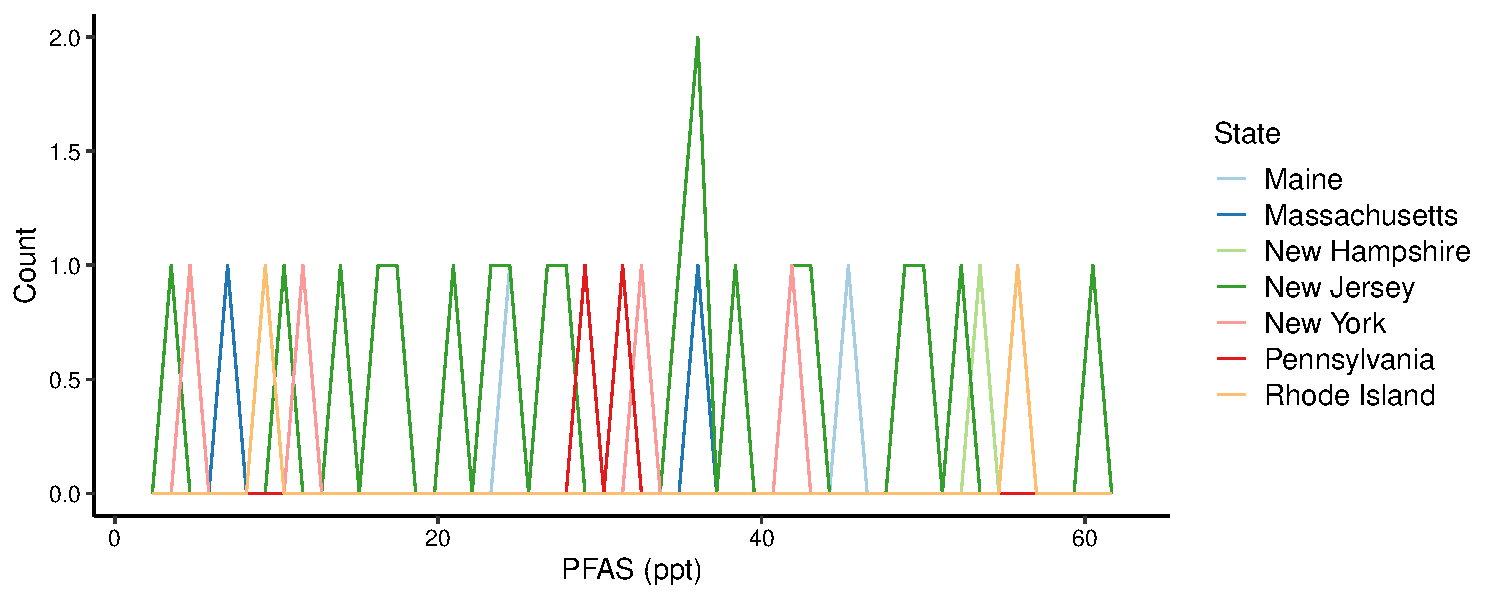
\includegraphics{Project_Template_files/figure-latex/figs4-1.pdf}
\caption{Frequency of PFAS Concentration Data in Noutheastern states.}
\end{figure}

\begin{quote}
Results from plots here**** and talk about how very little PFAS data
shown in these exploratory plots was the rationale behind doing this
analysis on the side, not i the geographic groupings here beceause
otherwise not enough data!!!!
\end{quote}

\newpage

\hypertarget{case-studies-data-exploration-for-north-carolina-and-massachusetts}{%
\subsection{Case Studies: Data Exploration for North Carolina and
Massachusetts}\label{case-studies-data-exploration-for-north-carolina-and-massachusetts}}

\begin{verbatim}
## Warning in as_grob.default(plot): Cannot convert object of class data.frame into
## a grob.
\end{verbatim}

\begin{verbatim}
## Warning: Removed 2865 rows containing non-finite values (stat_smooth).
\end{verbatim}

\begin{verbatim}
## Warning: Removed 2865 rows containing missing values (geom_point).
\end{verbatim}

\begin{verbatim}
## Warning: Removed 2810 rows containing non-finite values (stat_smooth).
\end{verbatim}

\begin{verbatim}
## Warning: Removed 2810 rows containing missing values (geom_point).
\end{verbatim}

\begin{verbatim}
## Warning: Graphs cannot be horizontally aligned unless the axis parameter is set.
## Placing graphs unaligned.
\end{verbatim}

\begin{figure}
\centering
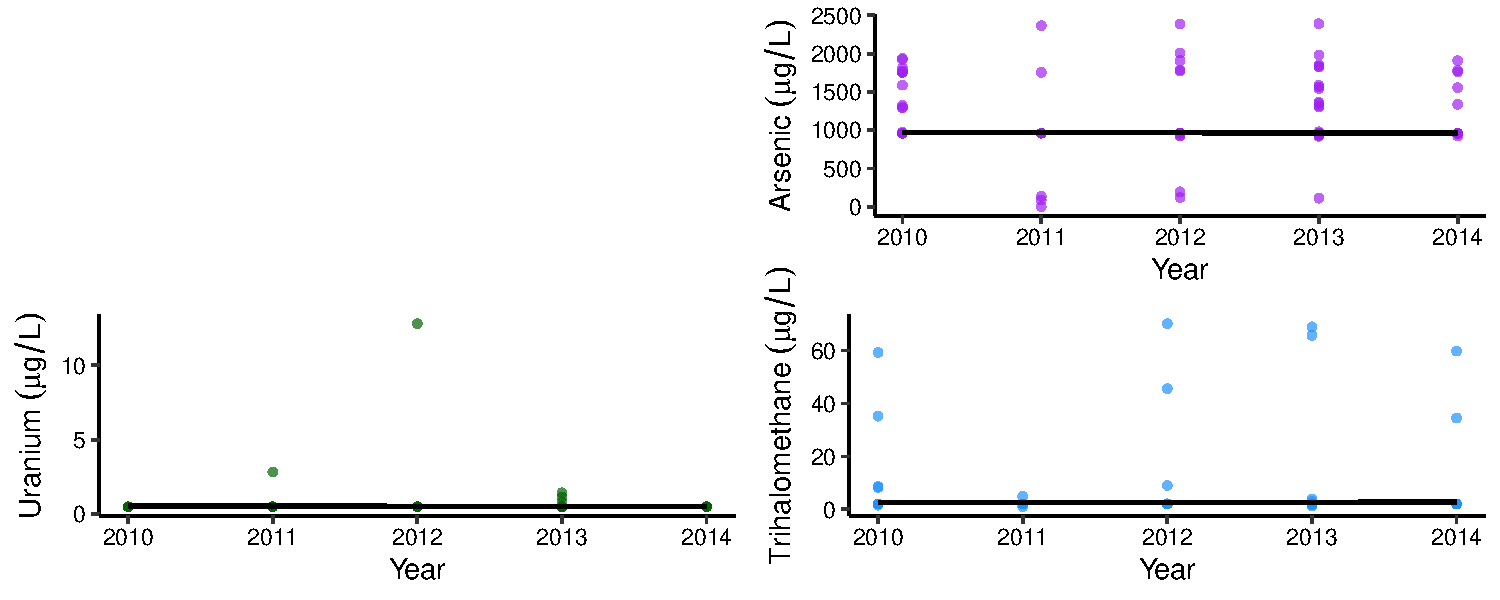
\includegraphics{Project_Template_files/figure-latex/figs5-1.pdf}
\caption{Water contaminant concentrations over time in North Carolina.}
\end{figure}

\begin{verbatim}
## Warning in as_grob.default(plot): Cannot convert object of class data.frame into
## a grob.
\end{verbatim}

\begin{verbatim}
## Warning: Removed 3509 rows containing non-finite values (stat_smooth).
\end{verbatim}

\begin{verbatim}
## Warning: Removed 3509 rows containing missing values (geom_point).
\end{verbatim}

\begin{verbatim}
## Warning: Removed 3321 rows containing non-finite values (stat_smooth).
\end{verbatim}

\begin{verbatim}
## Warning: Removed 3321 rows containing missing values (geom_point).
\end{verbatim}

\begin{verbatim}
## Warning: Graphs cannot be horizontally aligned unless the axis parameter is set.
## Placing graphs unaligned.
\end{verbatim}

\begin{figure}
\centering
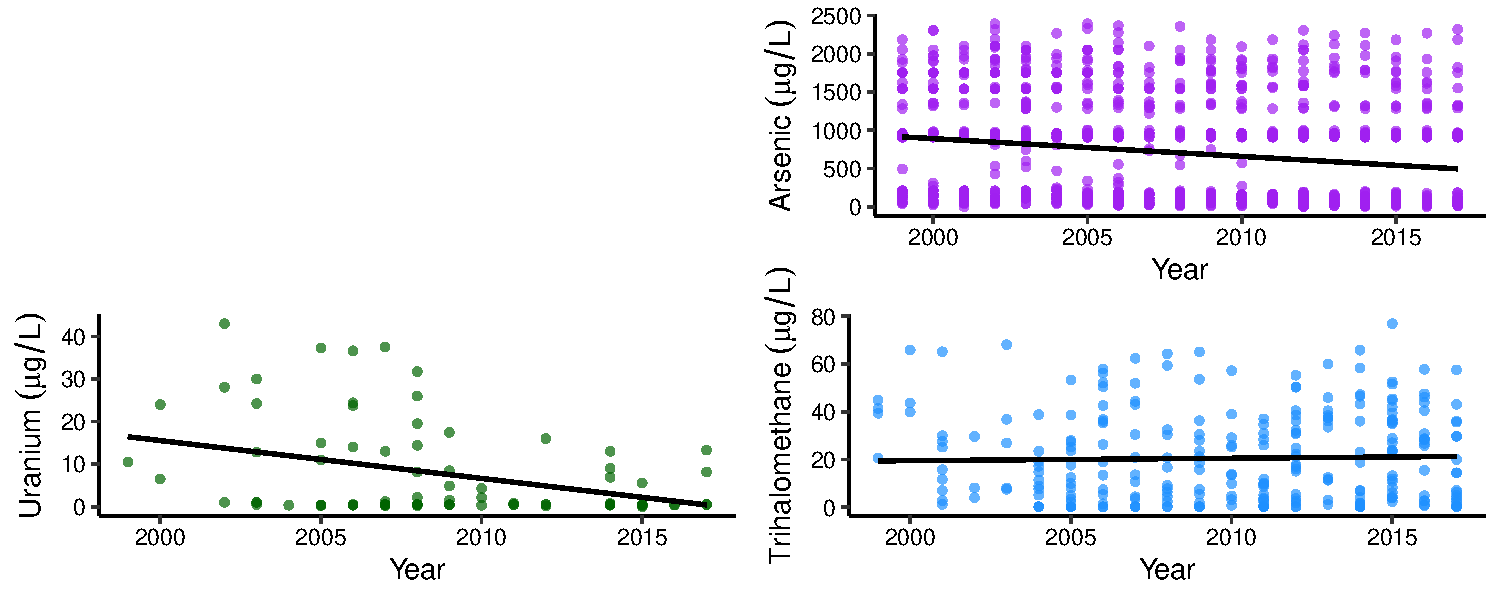
\includegraphics{Project_Template_files/figure-latex/figs6-1.pdf}
\caption{Water contaminant concentrations over time in Massachusetts.}
\end{figure}

\begin{quote}
Write findings here!! Relatively flat trend for all three contaminants
over 19 year period of data collection for NC, whereas uranium in MA
over time seems to be decreasingn, trihalo is slightly increasing, and
arsenic decreasing on average though still very high concentratiosn
\end{quote}

\newpage

\hypertarget{analysis}{%
\section{Analysis}\label{analysis}}

\hypertarget{question-1-do-arsenic-concentrations-vary-significantly-from-state-to-state-in-northeastern-and-southeastern-states}{%
\subsection{Question 1: Do arsenic concentrations vary significantly
from state to state in northeastern and southeastern
states?}\label{question-1-do-arsenic-concentrations-vary-significantly-from-state-to-state-in-northeastern-and-southeastern-states}}

\begin{figure}
\centering
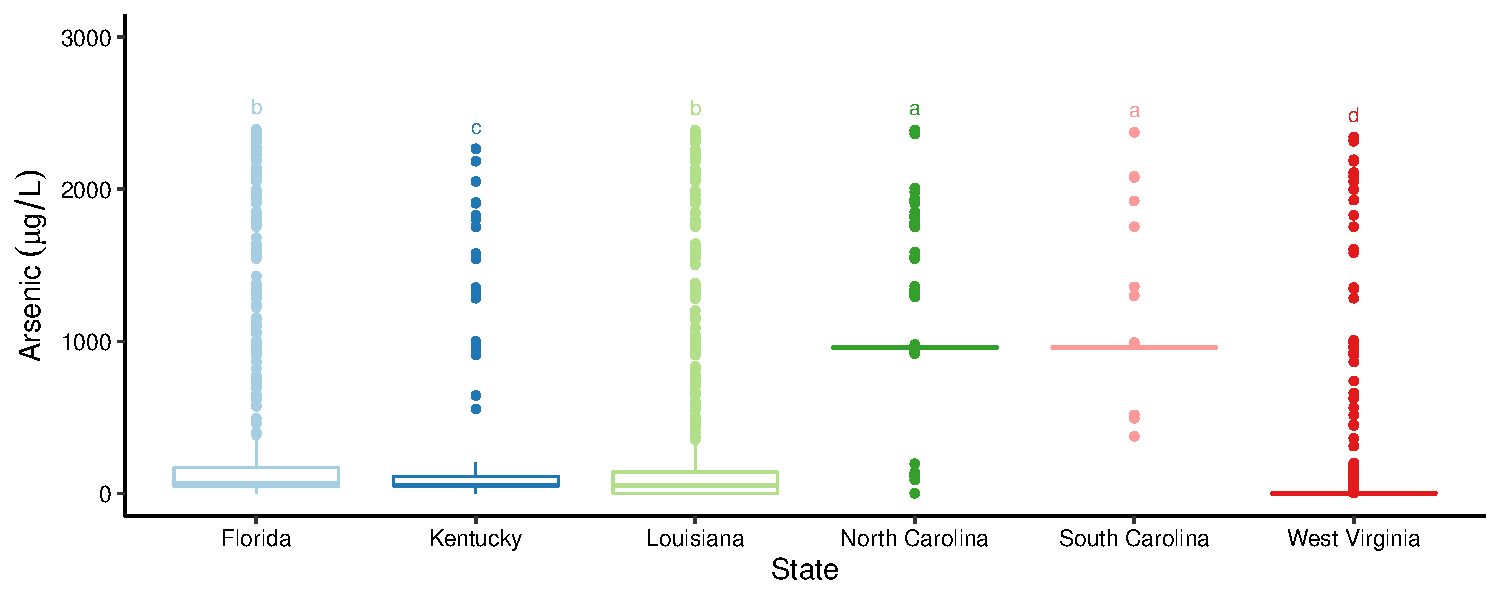
\includegraphics{Project_Template_files/figure-latex/figs7-1.pdf}
\caption{State by state comparison of arsenic values for southeastern
states.}
\end{figure}

\begin{quote}
Mean annual arsenic concentrations differ significantly between states
in the southeast (ANOVA; df=5, F=2872, p \textless{}0.0001). Mean
arsenic concentrations in West Virginia were significantly lower than in
other states and those in North Carolina and South Carolina were
significantly higher than those in other states (Post-hoc Tukey test;
Figure 7).
\end{quote}

\begin{figure}
\centering
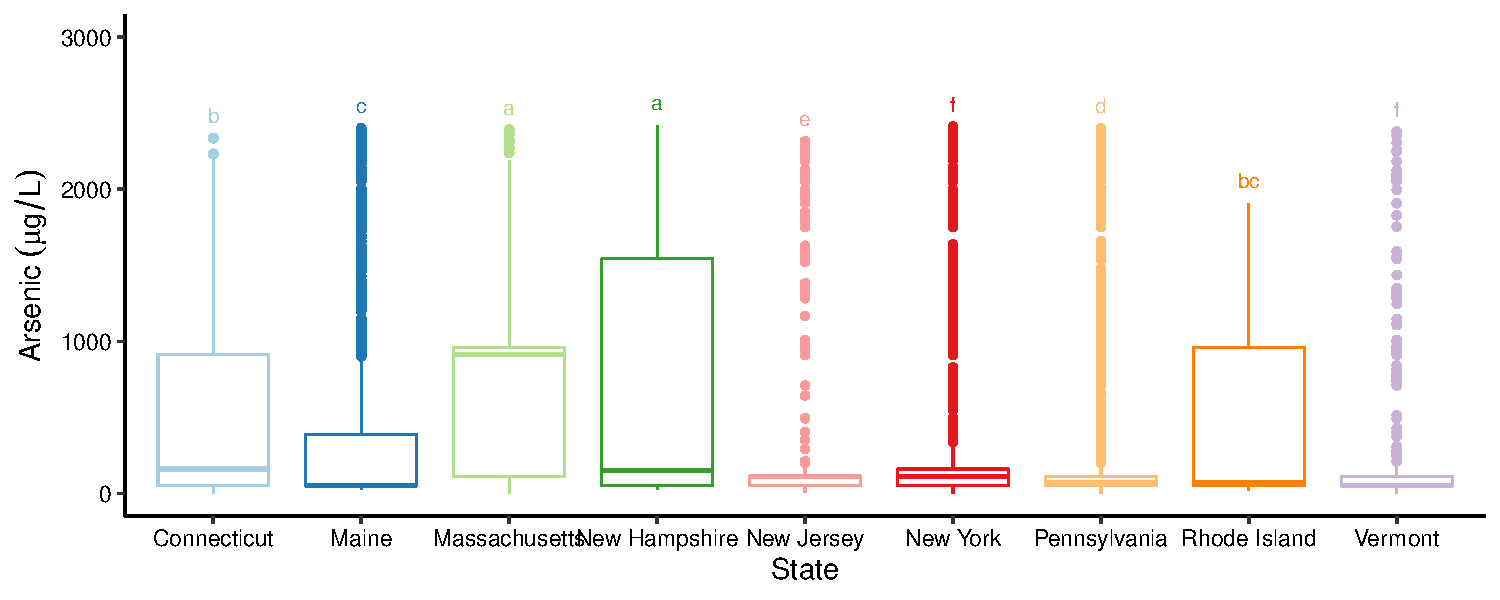
\includegraphics{Project_Template_files/figure-latex/figs8-1.pdf}
\caption{State by state comparison of arsenic values for northeastern
states.}
\end{figure}

\begin{quote}
Meaan annual arsenic concentrations also differ significantly between
states in the northeast (ANOVA; df=8, F=630.9, p\textless{}0.0001). Mean
arsenic concentrations in New York and Vermont were significantly lower
than in other states and those in New Hampshire and Massachusetts were
significantly higher than those in other states (Post-hoc Tukey test;
Figure 8).
\end{quote}

\hypertarget{question-2-do-socioeconomic-factors-or-the-presence-of-other-contaminants-predict-arsenic-concentrations-in-massachusetts-and-north-carolina}{%
\subsection{Question 2: Do socioeconomic factors or the presence of
other contaminants predict arsenic concentrations in Massachusetts and
North
Carolina?}\label{question-2-do-socioeconomic-factors-or-the-presence-of-other-contaminants-predict-arsenic-concentrations-in-massachusetts-and-north-carolina}}

\begin{quote}
For both states, uranium was explored as an explanatory variable but was
ultimately removed from both models for improved parsimony. Final
variables included to explain arsenic concentration included
trihalomethane concentration, MHI, and population served by the CWS for
both states.
\end{quote}

\begin{figure}
\centering
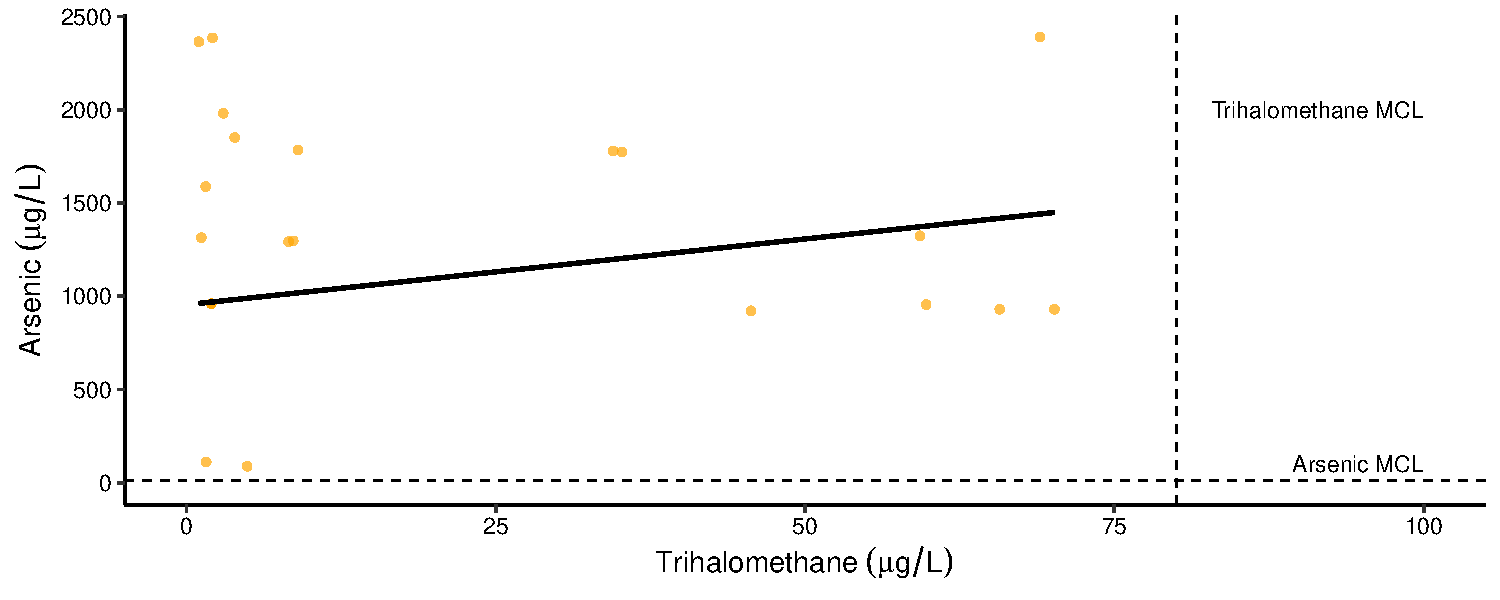
\includegraphics{Project_Template_files/figure-latex/figs9-1.pdf}
\caption{North Carolina Arsenic Concentrations by Population Served by
CWS Across Income Levels.}
\end{figure}

\begin{quote}
In North Carolina, population served by a CWS and trihalomethane
concentrations significantly predict arsenic concentrations, whereas MHI
is not a significant predictor of arsenic concentration (Multiple linear
regression; df=3 and 654, F=34.74, p\textless{}0.0001). Inreasing
arsenic concentration is associated with increasing trihalomethane
concentration and with decreasing population size served by a CWS.
\end{quote}

\begin{verbatim}
## Warning: Removed 18 rows containing non-finite values (stat_smooth).
\end{verbatim}

\begin{verbatim}
## Warning: Removed 18 rows containing missing values (geom_point).
\end{verbatim}

\begin{figure}
\centering
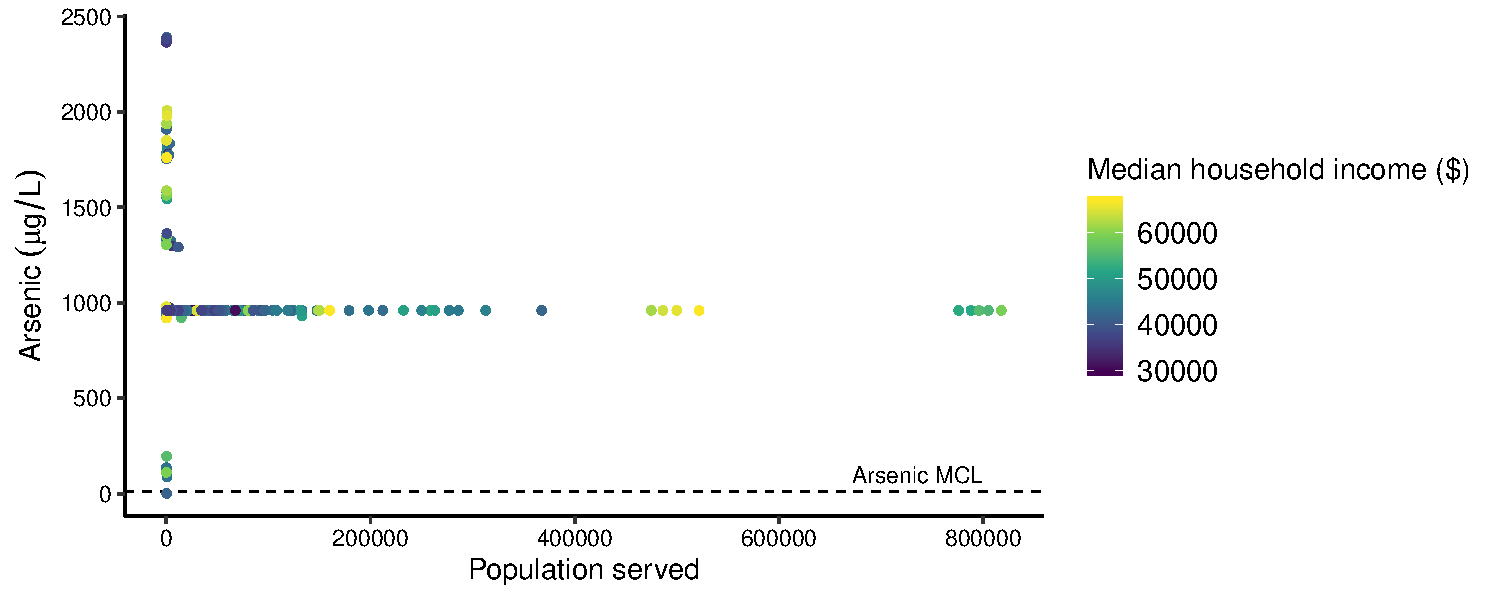
\includegraphics{Project_Template_files/figure-latex/figs10-1.pdf}
\caption{Massachusetts Arsenic Concentrations by Population Served by
CWS Across Income Levels.}
\end{figure}

\begin{quote}
In Massachusetts, population served by a CWS, trihalomethane
concentrations, and MHI do not significantly predict arsenic
conncentrations (Multiple linear regressio; df=3 annd 242, F-1.664,
p=0.1753). Figure 9 \ldots{}..FINISH LATER!! TALK ABOUT WHAT MCLS are
and what they are set to!!!!!
\end{quote}

\begin{verbatim}
## Warning: Removed 2810 rows containing non-finite values (stat_smooth).
\end{verbatim}

\begin{verbatim}
## Warning: Removed 2810 rows containing missing values (geom_point).
\end{verbatim}

\begin{verbatim}
## Warning: Removed 3321 rows containing non-finite values (stat_smooth).
\end{verbatim}

\begin{verbatim}
## Warning: Removed 3321 rows containing missing values (geom_point).
\end{verbatim}

\begin{figure}
\centering
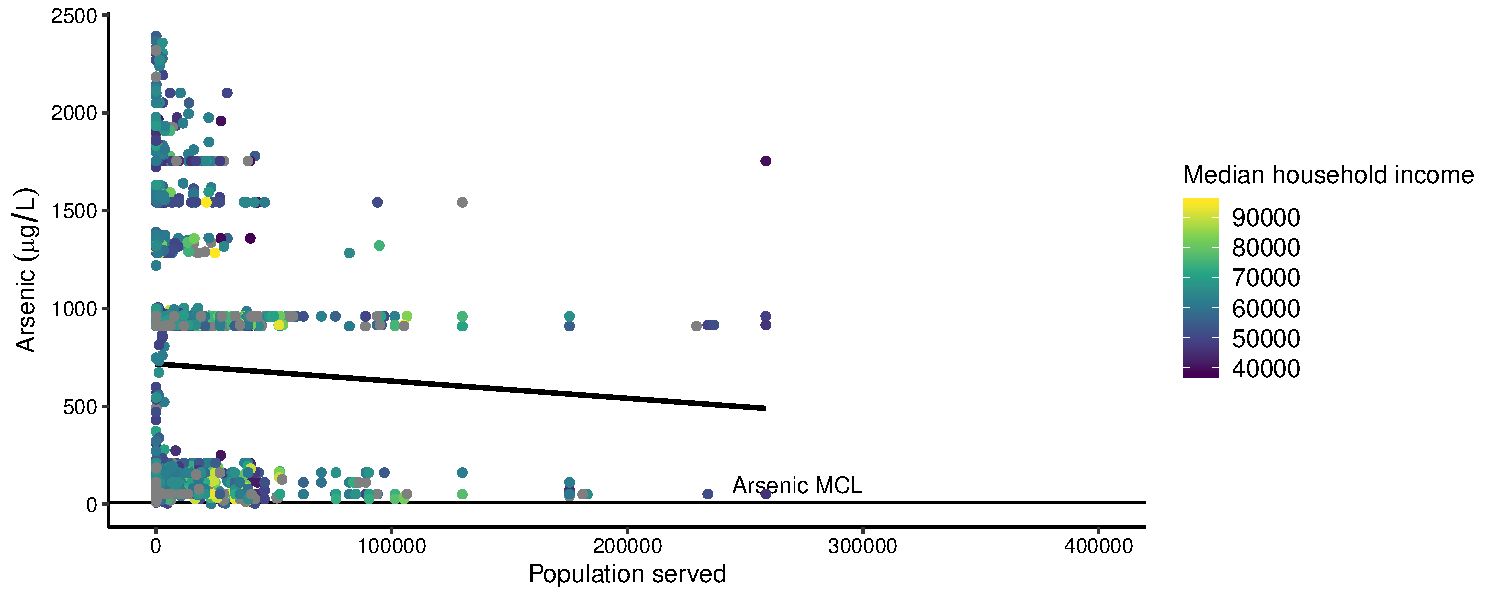
\includegraphics{Project_Template_files/figure-latex/figs11-1.pdf}
\caption{North Carolina v. Massachusetts: Arsenic Concentrations by
Trihalomethane Concentration.}
\end{figure}

\begin{quote}
TAKEAWAY HERE!
\end{quote}

\hypertarget{question-3.-do-pfas-concentrations-vary-signficantly-across-time-and-from-state-to-state-in-the-united-states-are-socioeconomic-factors-significant-predictors-of-pfas-concentrations}{%
\subsection{Question 3. Do PFAS concentrations vary signficantly across
time and from state to state in the United States? Are socioeconomic
factors significant predictors of PFAS
concentrations?}\label{question-3.-do-pfas-concentrations-vary-signficantly-across-time-and-from-state-to-state-in-the-united-states-are-socioeconomic-factors-significant-predictors-of-pfas-concentrations}}

\begin{quote}
Neither MHI nor population served by a CWS significantly predict PFAS
concentrations (Multiple linear regression; F=2 and 86, F=0.5912,
p=0.5559). An ANOVA was also run in preliminary analyses conducted for
PFAS data, but results are not included here due to issues with
missingness (25,938 observations were deleted when ANOVA was run).
TAKEAWAYS!
\end{quote}

\begin{verbatim}
## Warning: Removed 25946 rows containing non-finite values (stat_smooth).
\end{verbatim}

\begin{verbatim}
## Warning: Removed 25946 rows containing missing values (geom_point).
\end{verbatim}

\begin{figure}
\centering
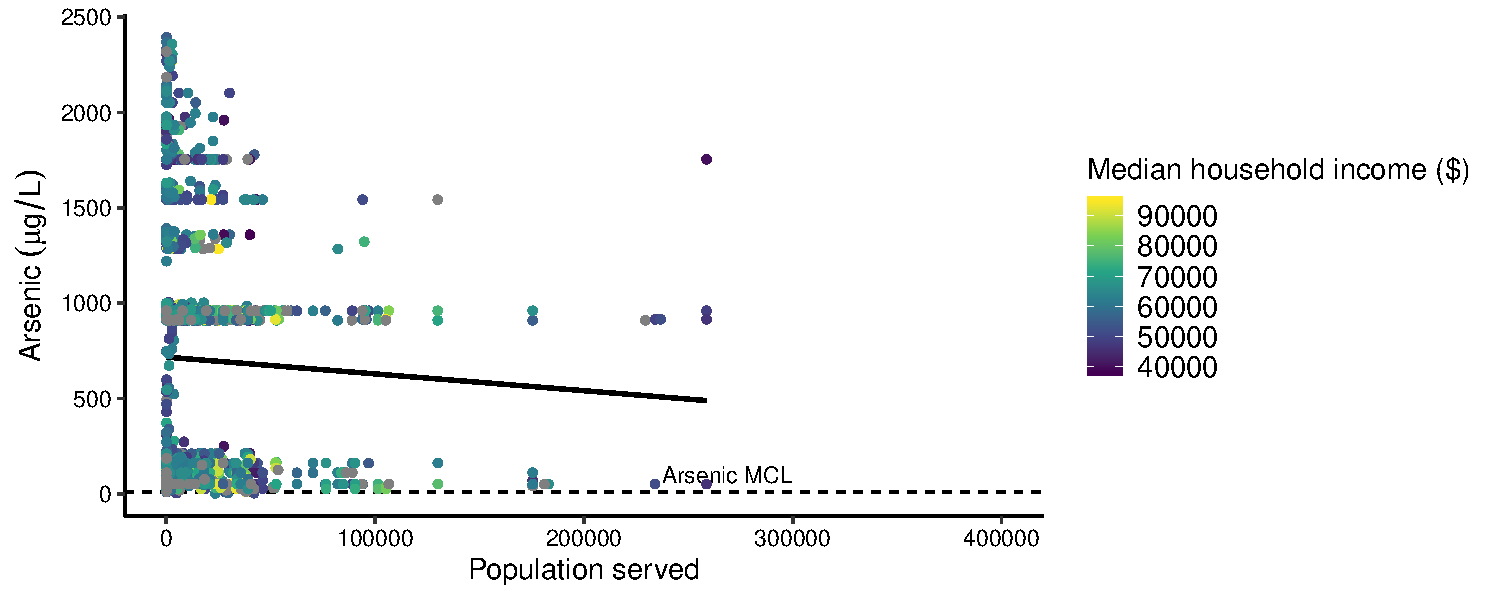
\includegraphics{Project_Template_files/figure-latex/figs12-1.pdf}
\caption{PFAS Concentration by Population Served by CWS Across Income
Levels.}
\end{figure}

\newpage

\hypertarget{summary-and-conclusions}{%
\section{Summary and Conclusions}\label{summary-and-conclusions}}

\begin{quote}
talk about conclusions and implications of findings\ldots{}and
supposition as to why these relationships exist Omitted variable bias:
R2s for all models were very low, talk about this Future: given scope of
project, couldn't possibly look in depth at each conntamiannt, so i nthe
future would be interested in exploring relationships for uranium and
TTHM such as those explored here for arsenic\ldots{}it's possible that
since arsenic is so ubiquitous inn geology that other contaminants could
have diff relationships with income for example\ldots{}
\end{quote}

\newpage

\hypertarget{references}{%
\section{References}\label{references}}

\begin{quote}
United States Environmental Protection Agency (USEPA). 2020. Safe
Drinking Water Act (SDWA). Retrieved from:
\url{https://www.epa.gov/sdwa}.
\end{quote}

\end{document}
